%%%%%%%%%%%%%%%%%%%%%%%%%%%%%%%%%%%%%%%%%%%%%%%%%%%%%%%%%%%%%%%%%%
%%%%%%%% ICML 2015 EXAMPLE LATEX SUBMISSION FILE %%%%%%%%%%%%%%%%%
%%%%%%%%%%%%%%%%%%%%%%%%%%%%%%%%%%%%%%%%%%%%%%%%%%%%%%%%%%%%%%%%%%

% Use the following line _only_ if you're still using LaTeX 2.09.
%\documentstyle[icml2015,epsf,natbib]{article}
% If you rely on Latex2e packages, like most moden people use this:
\documentclass{article}

% use Times
\usepackage{times}
\usepackage{amsmath}
\usepackage{amssymb}
% For figures
\usepackage{graphicx} % more modern
%\usepackage{epsfig} % less modern
\usepackage{subfigure} 

% For citations
\usepackage{natbib}

% For algorithms
\usepackage{algorithm}
\usepackage{algorithmic}

% As of 2011, we use the hyperref package to produce hyperlinks in the
% resulting PDF.  If this breaks your system, please commend out the
% following usepackage line and replace \usepackage{icml2015} with
% \usepackage[nohyperref]{icml2015} above.
\usepackage{hyperref}

% Packages hyperref and algorithmic misbehave sometimes.  We can fix
% this with the following command.
\newcommand{\theHalgorithm}{\arabic{algorithm}}

% Employ the following version of the ``usepackage'' statement for
% submitting the draft version of the paper for review.  This will set
% the note in the first column to ``Under review.  Do not distribute.''
\usepackage[accepted]{icml2015} 

% Employ this version of the ``usepackage'' statement after the paper has
% been accepted, when creating the final version.  This will set the
% note in the first column to ``Proceedings of the...''
%\usepackage[accepted]{icml2015}


% The \icmltitle you define below is probably too long as a header.
% Therefore, a short form for the running title is supplied here:
\icmltitlerunning{Correlations of correlations are not reliable statistics.}

\begin{document} 

\def\X{\mathbf{X}}
\def\x{\mathbf{x}}
\def\Y{\mathbf{Y}}
\def\L{\mathbf{L}}
\def\K{\mathbf{K}}
\def\N{\mathcal{N}}
\def\B{\mathbf{B}}
\def\E{\mathbf{E}}
\def\mbE{\mathbb{E}}
\def\t{\mathbf{t}}
\def\I{\mathbf{I}}
\def\H{\mathbf{H}}
\def\u{\mathbf{u}}
\def\beq{\begin{equation}}
\def\eeq{\end{equation}}
\def\BSig{\boldsymbol \Sigma}

\twocolumn[ \icmltitle{Correlations of correlations are not reliable
    statistics: \\ implications for multivariate pattern analysis. }

% It is OKAY to include author information, even for blind
% submissions: the style file will automatically remove it for you
% unless you've provided the [accepted] option to the icml2015
% package.

\icmlauthor{Bertrand Thirion}{bertrand.thirion@inria.fr}
\icmladdress{Parietal team, INRIA, Saclay and CEA, Neurospin France}
\icmlauthor{Fabian Pedregosa}{}
\icmladdress{CEREMADE/Chaire Havas-Dauphine \'Economie des Nouvelles Don\'ees}
\icmlauthor{Michael Eickenberg}{}
\icmladdress{Parietal team, INRIA, Saclay and CEA, Neurospin France}
\icmlauthor{ Ga\"el Varoquaux}{}
\icmladdress{Parietal team, INRIA, Saclay and CEA, Neurospin France}

% You may provide any keywords that you 
% find helpful for describing your paper; these are used to populate 
% the "keywords" metadata in the PDF but will not be shown in the document
\icmlkeywords{Statistics, permutation tests, heteroscedasticity, pattern analysis, representational similarity analysis, linear models.}

% You may provide any keywords that you 
% find helpful for describing your paper; these are used to populate 
% the "keywords" metadata in the PDF but will not be shown in the document

\vskip 0.3in
]

\begin{abstract}
Representational Similarity Analysis is a popular framework to
flexibly represent the statistical dependencies between multi-voxel
patterns on the one hand, and sensory or cognitive stimuli on the
other hand.
%
It has been used in an inferential framework, whereby significance is
given by a permutation test on the samples.
%
In this paper, we outline an issue with this statistical procedure:
namely that the so-called pattern similarity used can be influenced by
various effects, such as noise variance, which can lead to inflated
type I error rates.
%
What we propose is to rely instead on proper linear models.
\end{abstract} 

\section{Introduction}
\label{introduction}
% canonical framework: encoding and decoding.
The use of machine learning in functional neuroimaging has been
boosted in the recent years by the adoption of the so-called
\textit{multivariate pattern analysis} (MVPA) framework, in which
brain activation signals are compared to stimuli using multivariate
models such as \cite{Haxby2001,Cox2003,Haynes2006}.
%
More precisely, two settings have emerged to draw statistically
meaningful conclusions regarding the statistical associations between
experimental stimuli and brain activation measurements: 
%
On the one hand, \textit{encoding models} define a mapping from
possibly very high-dimensional features extracted from the stimuli to
brain activity at a given location.
%
On the other hand, \textit{decoding models} test whether the activity
in a given set of voxels --possibly the whole brain-- are predictive of
a certain feature of the stimuli used during the acquisition.
%
These two settings have been clearly described in
e.g. \cite{Naselaris2011,varoquaux:hal-01094737}.
%
The popularity of this framework is notably driven by the premise to
offer a more sensitive detection of task-related brain activations,
due to the pooling effect on voxels (decoding) or on stimulus features
(encoding).
%
In the present work we focus on functional Magnetic Resonance Imaging
(fMRI) data.

% new framework: RSA: avoid explicit model between stimuli and activity.
An alternative to these two models has been proposed, which borrows
from both ideas: it consists in quantifying the between-sample
similarity of the stimuli on the one hand and of the evoked activation
signals on the other hand, in order to find whether there is some
common structure between these two sets of similarities. 
%
% XXX Michael: One could also allude to the fact that RSA is a symmetric
% XXX approach like CCA
% XXX Bertrand: I have this in mind, but I prefer to keep this short 
% and focussed. But this should be part of a paper.  
%
This approach has been called \textit{Representational Similarity
  Analysis} (RSA) \cite{Kriegeskorte2008,Kriegeskorte2009} and is also
very popular.
%
A striking aspect is that, unlike
encoding and decoding models that require algorithmically or
computationally involved estimators, RSA simply relies on descriptive
statistics of the data, making it conceptually simple and affordable.

% pros and cons of RSA.
A discussion of the motivation for RSA can be found in \cite{Nili2014}:
%
On the one hand, this approach offers a great flexibility in terms of
experimental design, and is easy to implement and use.
%
It is also viewed as a sensitive statistic to detect associations
between stimuli and brain activity (see e.g. \cite{borghesani:hal-00986606}).
%
On the other hand, this approach does not rely on any signal model;
unlike more classical encoding and decoding, it actually avoids
defining explicit associations between brain patterns and combinations
of stimuli. 
%
In that sense, it can be viewed as a \textit{black box} model.

% Our contribution: a criticism of RSA based on statistical arguments (model, simulations and experimental data).
It is fair to consider that there are two main parts to RSA: one is
the representation of similarities of the input stimuli and the second
part compares it to neuroimaging data correlation.
%
In this work, we discuss the second part, namely the comparison
between RSA and linear encoding models. 
%
We outline the convergence between the two approaches, but also some
important differences that should be taken into account when
discussing the results of statistical analysis based on RSA.
%
Our contribution consists of a discussion of the model, followed by
illustrative experiments on simulated and experimental data.
%
Our main finding is that, in spite of the use of non-parametric
statistics, RSA-based inference is not reliable, because it can be
sensitive to effects that are not stimulus-related signals increase
(or decrease).
%
To give a simple perspective, we only consider the simplest setting
where RSA can be compared to alternative encoding schemes.
% for the sake
%of detecting some statistical associations between stimuli and
%regional brain activity.


\section{Statistical inference in RSA}
\label{rsa}
% expose the model
% comparison with linear model
% shortcoming
\subsection{Representational Similarity Analysis}
% XXX Michael: Wouldn't one classically put X\in\R^{n\times p} and
% XXX set the number of voxels as q?
% 
Let $\Y$ be an fMRI dataset, written as an $n \times p$ matrix, where
$n$ is the number of samples and $p$ is the number of voxels, possibly
after reduction to a particular Region of Interest.
%
Note that $n$ can be the number of acquired images %resolution 
or the result
of a deconvolution step.
%
This dataset is associated with an experimental paradigm, represented
by a succession of $n$ stimuli presentations.
%
One can represent it with a design matrix $\X$ of
shape $(n, q)$, where $q$ is the number of stimulus features or directly
with a kernel matrix $\K$ of size $n \times n$ that represents some
kind of similarity between the stimuli.
%
In this work,we explicitly assume that both representations are
available, with $q<n$ and that $\K=\text{Corr}(\X)$.

Representational similarity analysis proceeds by extracting the
lower-triangular coefficients of the activation similarity matrix
$\text{Corr}(\Y)$, yielding $\t_Y = \text{Tril} (\text{Corr}(\Y))$ and of the kernel $\t_X
=\text{Tril}(\K)$.  The decision statistic is Spearman correlation
between $\t_X$ and $\t_Y$. 
%
In the following derivation, we consider Pearson correlations instead
to simplify the analysis, but this is actually an arbitrary choice, and
we did not observe any significant difference in a real dataset (note
that in the experiments described later, we use Spearman correlation).
\beq R_{RSA} = \text{Pearson}/\text{Spearman}(\t_X, \t_Y)
\label{eq:spearman}
\eeq


\subsection{Statistical inference}
This basic RSA setting can be used to detect significant associations
between $\Y$ and $\X$ by using a permutation test: after shuffling
either $\Y$ or $\X$ in the sample dimension $J$ times, with
e.g. $J=10^4$, the distribution of the permuted Spearman correlation
$(R_{RSA}^j)_{j \in [J]}$ is computed and the initial value $R_{RSA}$
in eq. \ref{eq:spearman} is compared with $(R_{RSA}^j)_{j \in [J]}$,
where the proportion of higher values in the permuted sample is the
p-value.

\subsection{Comparison with encoding model}
The encoding formulation is obtained through the following
mass-univariate model:
\beq
\Y = \X\B + \E,
\label{eq:lm}
\eeq where $\B$ is $q \times p$ matrix that represents the response in
each voxel.  For instance, if $\X$ is the occurrence matrix of a
stimulus belonging to a set of discrete classes, $\B$ are the
univariate effects of an ANOVA model.
%
Here we assume that $q \ll n$, so that one can resort to simple
least-squares estimators.
%
The natural decision statistic of the linear model \eqref{eq:lm} is the
residual sum of squares of the residuals, which is a monotonous
function of the following $R^2$ quantity:
\beq R^2 = Tr(\X\hat{\B}\hat{\B}^T\X^T)\eeq
\begin{equation*} = Tr(\X\B\B^T\X^T) + Tr(\X\X^\dag\E\E^T)
+2 Tr(\X\X^\dag\E\B^T\X^T),
\end{equation*} where
$\X^\dag$ is the pseudo-inverse of $\X$; the third term can be
neglected as it has a null expected value. The remaining error term is
actually the squared norm of the projection of $\E$ on the span of the
design matrix column vectors.


\subsection{Statistical issues with RSA}
Using the previous generative model, a rudimentary data kernel,
without centering or normalization, is given by:
% XXX Michael: The LHS is symmetric whereas the RHS is not. The formula would
% XXX be correct if trace is taken on both sides. Like this it has to be
% XXX \Y\Y^T = \X\B\B^T\X^T + \E\E^T + \X\B\E^T + \E\B^T\X^T
\begin{equation*} \Y\Y^T = \X\B\B^T\X^T + \E\E^T + \X\B\E^T + \E\X^T\B^T 
\end{equation*}
from which one can compute the correlation matrix of $\Y$, after 
centering and normalization of the voxel time series, which yields:
\begin{equation*}
%\mbE(\Y\Y^T\X\X^T) = Tr(\X\B\B^T\X^T\X\X^T) + Tr(\mbE(\E\E^T)\X\X^T)
\widehat{\text{Corr}}(\Y) = \Delta_{\Y}^{-\frac{1}{2}} \H\Y\Y^T\H
\Delta_{\Y}^{-\frac{1}{2}},
\end{equation*}
where $\H$ is the centering matrix $\H=\I_n - \frac{1}{n}\u\u^T$,
  $\u$ being the unit vector, and $\Delta_\Y$ is the diagonal
  matrix with the same diagonal as $\H\Y\Y^T\H$

To go one step further, one can further assume that the voxels in the
region of interest share the same %
% XXX Michael: I would suggest saying "sample covariance matrix"
% XXX in order to disambiguate from a spatial one in a matrix-variate
% XXX Gaussian setting. 
 covariance matrix $\BSig$ (in the sample dimension). Let us also
 assume that the null hypothesis is true, i.e. that the effect $\B$ is
 null.
%
It follows that $\mbE(\Y\Y^T) = p\BSig$. Hence,
% XXX Michael: This is centering and normalizing in the sample axis. For the
% XXX same operation in the feature axis the operators would need to stand
% XXX between the Y and YT
\beq \widehat{\text{Corr}}(\Y) \rightarrow \Delta_{\BSig}^{-\frac{1}{2}} \H\BSig\H
\Delta_{\BSig}^{-\frac{1}{2}}\eeq 
in the large $p$ limit, where $\Delta_{\BSig}$ is the diagonal
  matrix with the same diagonal as $\H\Sigma\H$.  Given that
\beq 
R_{RSA} = \frac{1}{2}Tr\left((\widehat{\text{Corr}}(\Y) - \I) \K \right),\eeq
 the RSA statistic asymptotically reflects the non-diagonal terms of
$\Delta_{\BSig}^{-\frac{1}{2}} \H\BSig\H \Delta_{\BSig}^{-\frac{1}{2}}$.

\begin{figure}
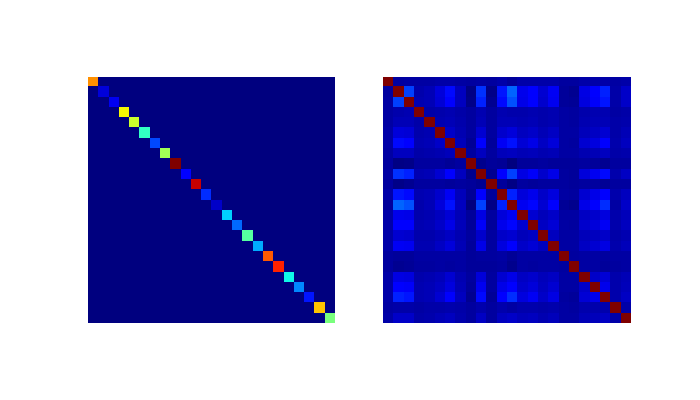
\includegraphics[width=\linewidth]{figures/covariance}
\caption{Heteroscedasticity and non-diagonal correlation matrix:
  (left) a generic diagonal matrix covariance $\BSig$ yields a non
  diagonal correlation matrix (right) due to centering of $\Y$ across
  samples and the normalization of correlation values.}
\label{fig:covariance}
\end{figure}


The key point is that, even if $\BSig$ is diagonal, the centered and
normalized matrix is not (see Fig. \ref{fig:covariance}). 
%
Hence, owing to the structure of $\BSig$, it can be positively or
negatively correlated with $\K$, leading to positive or negative
correlations.
%
By contrast, under the null hypothesis, the linear
model statistic converges asymptotically to $Tr(\X\X^\dag\BSig)$
and thus measures the proportion of variance in $\BSig$ that is fit
by span($\X$), without any additional bias.
%
This means that the RSA decision is sensitive to heteroscedasticity of
the noise, namely the fact that the noise varies across
conditions/voxels. 
%
However, such variations are not unexpected, due to the artefactual
effects that affect the BOLD signal (motion, tiredness, fluctuations
in vigilance), yet they should not be confused with actual
task-related BOLD signal increases.


\section{Experiments and results}
In a simulation experiment, we first exhibit the kind of issue that
can affect RSA type inference in heteroscedastic noise. We then
turn to a real dataset and show that the heteroscedasticity issue is
actually not negligible.

\subsection{Simulated data}
We generate a simplistic dataset, where $p=100$ voxels are observed
during the occurrence of a certain paradigm with $n=24$ samples. The
paradigm is simply assumed to be a linear function of the sample
number.
%
We rely on two Gaussian noise models: one i.i.d., hence %can be said
\textit{homoscedastic}; the second one %is 
heteroscedastic, with
variance increased by a factor of 2 for the second half of the
samples.
%
Note that these fluctuations are not perfectly correlated with the
assumed paradigm and cannot be viewed as a functional signature.
% 
The $R_{RSA}$ and $R^2$ statistics are evaluated, and the
statistical significance is computed with a permutation test with
$J=10^4$ permutations. The experiment is repeated $10^3$ times. We
present a histogram of these p-values in Fig \ref{fig:sim}. Note that
these histograms are expected to be flat, because no effect was
simulated.

\begin{figure}[t]
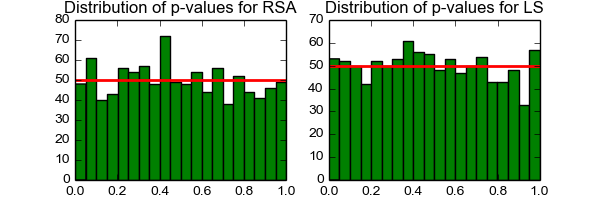
\includegraphics[width=\linewidth]{figures/rsa_specificity_homo.png}
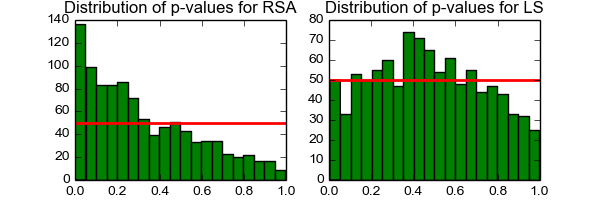
\includegraphics[width=\linewidth]{figures/rsa_specificity_hetero.png}
\caption{Results of the simulation under the null hypothesis:
  histogram of the p-values. (Top) under homoscedastic noise
  conditions, the distribution of the p-values under the null
  hypothesis is flat. (Bottom) under heteroscedastic conditions, the
  distribution becomes non-flat both for RSA and the linear
  model. However, the accumulation of very low p-values occurs only
  for RSA, meaning that the false positive rate is no longer under
  control.}
\label{fig:sim}
\end{figure}

Indeed, under homoscedastic noise conditions, the distribution of the
p-values under the null hypothesis is flat. By contrast, under
heteroscedastic conditions, the distribution becomes non-flat both for
RSA and the linear model. However, the accumulation of very low
p-values occurs only for RSA, meaning that the false positive rate is
no longer under control, while the linear model does not yield too
many low p-values.

\subsection{Experimental data}

We use the dataset described in \cite{Haxby2001}, in which subjects
were viewing images from 8 different categories (shoes, bottles,
places, faces, cats, scissors, scrambled pictures). We study the
representation of these categories in the visual cortex by using a
predefined parcellation using the Harvard-Oxford atlas, split between
hemispheres (96 regions).
%
We obtain the p-values of the association test between conditions by
using either a linear model or an RSA approach, by computing the
statistics defined previously and a permutation test (where the labels
are shuffled %randomly 
across sessions, but the within-session block
structure is preserved), with $J=10^4$ permutations.
%
In parallel, we display the result of a Fligner test that detects
variance difference across blocks.
%
We used different chunks of 4 sessions in one subject, and obtained
similar outcomes: we display in Figure \ref{fig:haxby} their result with
sessions 1-4 of subject 1.
%
We rely on Nilearn functions for fetching the data, the atlas and
the visualization \cite{Abraham2014}.

\begin{figure}[t]
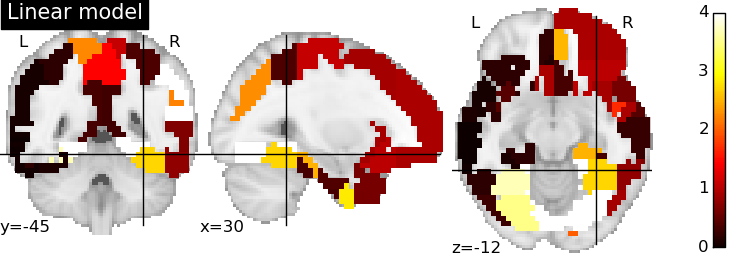
\includegraphics[width=\linewidth]{figures/lm.png}
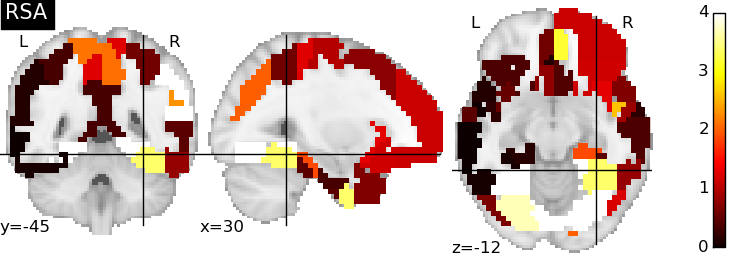
\includegraphics[width=\linewidth]{figures/rsa.png}
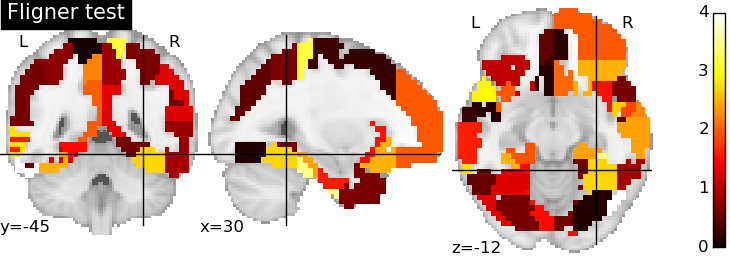
\includegraphics[width=\linewidth]{figures/var_stat.png}
\caption{ Differences between RSA and linear encoding models and noise
  heteroscedasticity.  (Up) $\log_{10}p$-value of the encoding
  approach based on a linear model; (middle) $\log_{10}p$-value of the
  RSA test (down) $\log_{10}p$-value of the Fligner test that detects
  difference of variances across blocks. While the RSA and encoding
  model yield mostly similar results, there is a difference of
  significance e.g. in the anterior fursiform gyrus; in parallel, one
  observe significant variance fluctiations with the Fligner
  test.}
\label{fig:haxby}
\end{figure}

One can observe that in general, the RSA and encoding model yield
qualitatively similar results, with higher response in the occipital
cortex and right orbitofrontal cortex. 
%
There are also some differences, with more significant values for RSA,
such as in the right anterior fusiform gyrus, but this is associated
with significant variance fluctuations across blocks, which calls for
some caution when interpreting the results in this area.

\section{Conclusion}
The present work aimed at \textit{i)} recalling the fact that RSA
analysis can in many settings be handled using explicit linear
encoding models \textit{ii)} uncovering some differences between the
significance of associations observed using encoding models and RSA,
where the main difference lies in the way to handle the neuroimaging
data: an explicit linear fit in the case of encoding model (possibly
regularized if necessary), against a comparison of correlation
structures of RSA.
%
The latter, implicit approach suffers from the ill-controlled behavior
of correlations, e.g. when the data are not i.i.d in the time/sample
dimension.
%
For the sake of simplicity, we assumed a relatively simple structure of
the set of stimuli: namely that of a low-rank model (i.e. a design
matrix with few columns). 
%
However, we acknowledge that this does not represent all possible use
cases and defer the investigation of more complex analyses (full rank
square design matrices) to future work.

Finally, it should be emphasized that the cognitive problems to be
addressed are usually much more subtle than those discussed here. 
%
For instance, they may involve the use of several concurrent variables,
where the selective association of some of them with the neuroimaging
data has to be established.
%
However, permutation testing with multiple independent variables is
notoriously hard to handle in the case of linear models
\cite{Anderson2001}, hence arguably more problematic with RSA.

\section*{Acknowledgement}
The research leading to these results has received funding from the
European Union Seventh Framework Programme (FP7/2007-2013) under grant
agreement n° 604102 (HBP), from the joint Inria-Microsoft Research lab
(\textit{MediLearn} project) and from the ANR funding agency,
BrainPedia project ANR-10-JCJC 1408-01.

\bibliography{rsa}
\bibliographystyle{icml2015}

\end{document} 


% This document was modified from the file originally made available by
% Pat Langley and Andrea Danyluk for ICML-2K. This version was
% created by Lise Getoor and Tobias Scheffer, it was slightly modified  
% from the 2010 version by Thorsten Joachims & Johannes Fuernkranz, 
% slightly modified from the 2009 version by Kiri Wagstaff and 
% Sam Roweis's 2008 version, which is slightly modified from 
% Prasad Tadepalli's 2007 version which is a lightly 
% changed version of the previous year's version by Andrew Moore, 
% which was in turn edited from those of Kristian Kersting and 
% Codrina Lauth. Alex Smola contributed to the algorithmic style files.  
